\section{\texorpdfstring{AutoLibra as a lens 
\includegraphics[height=1em]{figs/microscope.png}: agent evaluation with AutoLibra}{AutoLibra as a lens: agent evaluation with AutoLibra}}
\label{sec:lens}

In this section, we use AutoLibra as a lens to provide grounded, behavior-salient insights into agent trajectories. In three data sets, CoGym \citep{shao2024collaborative}, Sotopia \citep{zhousotopia}, and WebVoyager \citep{he2024webvoyager}, we compare induced metrics with heuristically proposed evaluation dimensions and failure modes summarized by the authors. We find that AutoLibra can discover more concrete metrics than heuristically defined categories, and novel metrics that are overlooked by experts. 

\begin{table}[!h]
\centering
\begin{tabular}{ll}
    \toprule
    AutoLibra\protect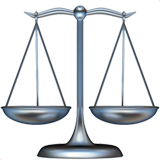
\includegraphics[height=1em]{figs/scale.png}-induced metrics & CoGym failure categories\\\midrule
    \multicolumn{2}{c}{Matched metrics and categories}\\\midrule
    \textit{Responsiveness and Efficiency} (75\%) & \textit{Communication} (65\%) \\
    \emph{Communication Clarity and Notification} (8\%) & \textit{Communication} (65\%)\\
    \textit{Instruction Adherence and Follow-Through} (24\%) & \textit{Situational Awareness} (40\%)\\
    \textit{Iterative Refinement and Adaptability} (47\%) & \textit{Planning} (39\%)\\
    \textit{Autonomy and Proactiveness} (28\%) & \textit{Planning} (39\%) \\
    \textit{Search and Retrieval Accuracy} (13\%) & \textit{Environmental Awareness} (28\%) \\
    \textit{Data Analysis Competence} (2\%) & \textit{Environmental Awareness} (28\%) \\
    \textit{Interface and User Experience} (23\%) & \textit{Personalization} (16\%) \\\midrule
    \multicolumn{2}{c}{Unmatched AutoLibra\protect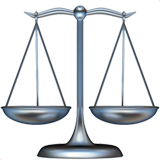
\includegraphics[height=1em]{figs/scale.png}-induced metrics}\\\midrule
     \multicolumn{2}{C{0.8\textwidth}}{\textit{Content Quality and Coherence} (16\%)} \\ \bottomrule
\end{tabular}
\caption{Comparison between AutoLibra-induced metrics and CoGym failure categories}
\label{tab:lens_cogym}
\end{table}

\paragraph{CoGym}
For CoGym \citep{shao2024collaborative}, AutoLibra induces 9 metrics from feedback from \textbf{end users}, of which 7 can be matched to the five failure categories by the CoGym authors. Both \textit{Responsiveness and Efficiency} and \textit{Content Quality and Coherence} overlap with the five failure categories. This shows that AutoLibra induces metrics that reflect human expert categorization, but also provides a different perspective to understand agent performance.

%\textit{Communication clarity and user interaction} belongs to Communication,  \textit{Adherence to instructions and consistency} belongs to Situational Awareness, \textit{Adaptability and responsiveness to feedback} belongs to Planning, \textit{Search accuracy and content relevance} belongs to Environment Awareness, and \textit{User preference query and incorporation} belongs to Personalization. All five metrics are more concrete and fine-grained than the larger categories in CoGym; we also discover the following metrics that are not mentioned in the break-down analysis in the CoGym paper:
%\textit{Responsiveness and Efficiency}, \textit{Content Quality and Coherence}, and \textit{Data Analysis Competence}. We note that this comparison shows the complementary characteristics of automatically 
%induced metrics, which are more concrete on the issues that users are noticing, while the expert-designed categories measure the high-level capabilities of AI agents. 

\begin{table}[!h]
\centering
\begin{tabular}{ll}
    \toprule
    AutoLibra\protect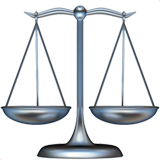
\includegraphics[height=1em]{figs/scale.png}-induced metrics & Sotopia-Eval dimensions\\
    \midrule
    \multicolumn{2}{c}{Matched metrics and dimensions}\\\midrule
    \textit{Goal Achievement and Outcome Effectiveness} & \textit{Goal Completion}\\
    \textit{Conversational Naturalness and Efficiency} & \textit{Believability} \\
    \textit{Contextual Integration of Identity} & \textit{Believability}\\
    \textit{Personality Consistency and Alignment} & \textit{Believability}\\ \midrule
    \multicolumn{2}{c}{Unmatched AutoLibra\protect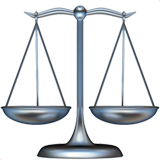
\includegraphics[height=1em]{figs/scale.png}-induced metrics}\\\midrule
     \multicolumn{2}{C{0.8\textwidth}}{\textit{Negotiation Tactics and Strategic Adaptability, Clarity and Precision in Communication, Responsiveness and Conversational Termination, Adaptability and Flexibility in Dialogue}} \\ \midrule
     \multicolumn{2}{c}{Unmatched Sotopia-Eval dimensions}\\\midrule
     \multicolumn{2}{C{0.8\textwidth}}{\textit{Relationship, Knowledge, Secret, Financial and Material Benefits, Social Rules}} \\\bottomrule
\end{tabular}
\caption{Comparison between AutoLibra-induced metrics and Sotopia failure categories \diyi{should we combine Table 2 and Table 3, Table 4? }}
\label{tab:lens_sotopia}
\end{table}

\paragraph{Sotopia} In Sotopia, we \citep{zhousotopia} proposed seven dimensions for evaluating social intelligence in AI agents. With AutoLibra, we recover the exact dimension \emph{Goal Completion}, and 3 metrics as the subdimensions of \emph{Believability}, indicating that \textit{Believability} could be too high-level, while AutoLibra provides more concrete breakdown metrics. 
AutoLibra induces another four metrics which are overlooked in the heuristically proposed Sotopia-Eval dimensions. We should note that the other five dimensions in Sotopia are still valuable evaluation dimensions for social intelligence. However, behaviors captured by \emph{Financial and Material Benefits}, \emph{Knowledge}, and \emph{Secret} dimensions are often also captured by \textit{Goal Completion} and \textit{Believability}. As a result, AutoLibra produces the single \textit{Goal Achievement and Outcome Effectiveness} metric through minimizing the redundancy. Whereas, \textit{Relationship} and \textit{Social Rules} captures long-tailed behaviors which are not picked up by AutoLibra.

\begin{table}[!h]
\centering
\begin{tabular}{ll}
    \toprule
    AutoLibra\protect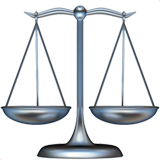
\includegraphics[height=1em]{figs/scale.png}-induced metrics & WebVoyager fail reasons\\
    \midrule
    \multicolumn{2}{c}{Matched metrics and dimensions}\\\midrule
    \textit{Navigation Accuracy} (11\%) & \textit{Navigation Stuck} (44\%) \\ 
    \textit{Access Barrier Handling} (2\%) & \textit{Navigation Stuck} (44\%)\\
    \textit{Error Recovery and Iterative Adjustment} (15\%) & \textit{Navigation Stuck} (44\%)\\
    \textit{Step Efficiency and Action Redundancy} (13\%) & \textit{Navigation Stuck} (44\%)\\ 
    \textit{Information Extraction and Verification Accuracy} (16\%) & \textit{Hallucination} (22\%)\\
    \textit{Result Relevance and Problem-Specific Accuracy} (9\%) & \textit{Prompt Misalignment} (9\%)\\
    \midrule
    \multicolumn{2}{c}{Unmatched AutoLibra\protect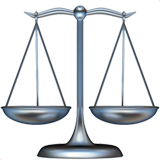
\includegraphics[height=1em]{figs/scale.png}-induced metrics}\\\midrule
     \multicolumn{2}{C{0.8\textwidth}}{\textit{Query and Search Strategy Efficiency} (7\%), \textit{Final Output and Summarization Quality} (18\%)}} \\ \midrule
     \multicolumn{2}{c}{Unmatched WebVoyager fail reasons}\\\midrule
     \multicolumn{2}{C{0.8\textwidth}}{\textit{Visual Grounding Issue} (25\%)} \\\bottomrule
\end{tabular}
\caption{Comparison between AutoLibra-induced metrics and WebVoyager failure categories}
\label{tab:lens_wv}
\end{table}

\paragraph{WebVoyager} Similarly, for web navigation tasks, AutoLibra also discovers metrics such as \textit{Access Barrier Handling}, \textit{Error Recovery and Iterative Adjustment}, \textit{Step Efficiency and Action Redundancy} which much more closely reflect emergent agent behavior than the failure analysis categories proposed in previous work \citep{he2024webvoyager,zhou2024proposeragentevaluatorpaeautonomousskilldiscovery}, where they are often simply classified as ``navigation stuck''; full results are tabulated in Table \ref{tab:lens_wv}. This further demonstrates AutoLibra's utility in extracting behavior-salient metrics, and particularly demonstrates its ability to obtain \textbf{fine-grained metrics} that expert design would not have been able to extract. 



